
\chapter{Reachability Analysis on Optimal Trim State for Aerial Docking}


Aerial refueling is an important capability to increase the endurance and flight range of aircraft, but it often suffers from a low success rate. The altitude and speed of the tanker aircraft in the docking phase play a great role in the docking success rate. According to this, the optimal trim state, namely the optimal speed and altitude of the tanker aircraft, is investigated through the reachability analysis method in this paper. The optimal problem is transformed to find the trim state corresponding to the maximum volume of the reachable set. First, a relative motion model of the receiver aircraft with respect to the drogue is proposed. Then, based on reachability analysis, an optimization problem is formulated and a solution procedure is given in detail. In the simulation, the volumes of reachable sets are plotted with respect to the given discrete speeds and altitudes, based on which the optimal trim state of the docking phase is determined. Finally, the determined optimal trim state is verified by using numerous docking control simulations and the degree of controllability from another aspect. The effectiveness of the proposed method is demonstrated.


\section{Introduction}

%Aerial Refueling (AR) is very important to military missions as it can
%extend the endurance and flight range of aircraft \cite{1}. During an AR
%process, the receiver aircraft first breaks away from its formation, then
%approaches the rear of the tanker aircraft for docking. Once the receiver
%aircraft completes refueling, the receiver aircraft disconnects with the
%tanker aircraft and rejoins the formation again. Therefore, the entire
%process can be decomposed into three phases: the approaching tanker phase,
%the docking phase, and the rejoin formation phase \cite{2}. This paper will
%focus on the docking phase which is the key step of an AR process.


Currently, AR processes are realized by experienced pilots of manned
aircraft or autopilots of Unmanned Aerial Vehicles (UAVs) which often suffer
from low success rates. In fact, inappropriate docking speeds and docking altitudes will affect the
docking success rate, but little attention has been paid. The related
references about existing chosen docking speeds and docking altitudes are
summarized in Table \ref{list_AV}. In \cite{3}, a deep learning based
trajectory optimization method was provided to decrease the bow wave effect on the drogue,
where the refueling altitude was set to be 7010 m and the speed of tanker aircraft was 200 m/s.
In \cite{4}, a back-stepping based flight controller for the receiver aircraft was designed,
where the speed of tanker aircraft was 200 m/s and the docking altitude was 7010 m.
In \cite{5}, an adaptive control method was used to reject the trailing
vortex, where the altitude was 1524 m and the docking speed was 152 m/s.
A command filtered backstepping sliding mode controller for the
hose whipping phenomenon in aerial refueling was designed in \cite{6}, where the refueling altitude and the speed of the tanker aircraft were set to be 7620 m and 200 m/s respectively.
The receiver forebody aerodynamic effect on the drogue transient motion was
considered in \cite{7}, where the speed of tanker aircraft was 118 m/s and
the docking altitude was 2286 m.
Furthermore, a lower order dynamic model involving the receiver forebody
aerodynamic effect was proposed to describe drogue dynamics in \cite{8},
where the docking altitude in this paper was set to be 3000 m and the
docking speed was 120 m/s.
In \cite{9}, a simple method was used to model
the receiver forebody aerodynamic effect, where the altitude of the tanker
aircraft was 3000 m and the docking speed was 120 m/s. The type of the
tanker aircraft is Boeing 707 and the receiver aircraft is F/A-18B.
In \cite{10}, the dynamic modeling and simulation application of the receiver
aircraft are studied, where the altitude of the tanker aircraft was 7010
m and the docking speed was 200 m/s.
In \cite{11}, the actual flight test
experiment was performed by NASA. The type of the tanker aircraft and the
receiver aircraft is F/A-18. The docking altitudes were 2286 m, 3200 m, 7620
m, 9144 m and the range of the docking speed was from 90 m/s to 152 m/s.
In \cite{12}, another NASA flight test experiment was made to reveal the forebody flow field of the receiver aircraft and two out of six capture attempts were successful. The capture criteria and miss criteria at the
docking phase were also provided. The type of the tanker aircraft is Boeing
707-300 and the type of the receiver aircraft is F/A-18. The docking
altitude and speed were both set to be constant. The actual flight test
experiments were also conducted by North Atlantic Treaty Organization
(NATO). In the ATP-56(B) issued by NATO \cite{13}, the tanker aircrafts are
VC-10 and KC-10, and receiver aircraft is F-16A. The altitude range for
refueling was from 1524 m to 6096 m and the speed range was from 118m/s to
165 m/s. By facing different docking speeds and altitudes, a problem arises
that what docking speed and altitude can make docking most easily. Motivated
by this, this paper aims at studying the optimal speed and altitude based on
the reachability analysis method. Concretely, different docking speeds and
altitudes will correspond to different volumes of the reachable set at the
docking phase, because they will change the relative motion model of the
receiver aircraft with respect to the center of the drogue. Therefore, the
speed and altitude corresponding to the maximum volume of reachable set are
regarded as the optimal trim state.

\begin{table}[ptb]
	\caption{Summary of the Simulation Experiments and the Actual Flight Test Experiments}
	\label{list_AV}%\begin{ruledtabular}
	\centering\setlength{\tabcolsep}{1mm}{ %
		\begin{tabular}{ccccc}
			\hline\hline
			Ref.  & The Tanker  & The Receiver  & Altitude  & Docking Speed \tabularnewline
			\hline
			\cite{3} & NA  & NA & $7010m$  & $200m/s$ \tabularnewline
			\hline
			\cite{4} & NA  & NA & $7010m$  & $200m/s$ \tabularnewline
			\hline
			\cite{5} & NA  & NA & $1524$  & $152m/s$ \tabularnewline
			\hline
			\cite{6} & NA  & NA & $7620$  & $200m/s$ \tabularnewline
			\hline
			\cite{7} & NA  & NA & $2286$  & $118m/s$ \tabularnewline
			\hline
			\cite{8} & NA  & NA & $3000m$  & $120m/s$ \tabularnewline
			\hline
			\cite{9} & Boeing 707 & F/A-18B & $3000m$  & $120m/s$ \tabularnewline
			\hline
			\cite{10} & NA  & NA & $7010m$  & $200m/s$ \tabularnewline
			\hline
			\cite{11} & F/A-18  & F/A-18 & $\begin{array}{c}
			2286,3200,\\
			7620,9144m
			\end{array}$ & $90\sim152m/s$ \tabularnewline
			\hline
			\cite{12} & Boeing 707-300  & F/A-18 & NA  & NA \tabularnewline
			\hline
			\cite{13} & VC-10, KC-10  & F-16A & $1524\sim6096m$  & $118\sim165m/s$ \tabularnewline
			\hline
	\end{tabular}}
\end{table}


It is reasonable to use the volume of the reachable set to measure how easy
the docking is. The subset of the state space that can reach the target set
while remaining in the acceptable range is called the reachable set \cite{14}%
. With respect to the docking phase, the target set represents the set of
successful docking states, and the reachable set is a set of the receiver
aircraft states from which the docking maneuver can be accomplished within a
finite time horizon. Thus, the larger the volume of the reachable set is,
the higher probability the pilot or the UAV autopilot can drive the receiver
aircraft to dock successfully. This further implies that it is more easily
to dock. So far, the reachability analysis method has been applied to solve
many problems, such as collision avoidance \cite{14}, control law design for
safe aerobatic maneuvers \cite{15} \cite{16}, safety verification of
autoland maneuvers \cite{17} and a ground moving target tracking \cite{18}.
In \cite{19}, the reachability analysis method was first applied to an AR
process. The AR process has been divided into several maneuver sequences and
the reachability analysis method was used to design a maneuver decision to
ensure safe operation of a sequential mode transition. Unlike \cite{19}, the
aim of this paper is to determine the optimal trim state of the docking
phase in terms of reachability.

The reachable set can be calculated by the Level Set Toolbox \cite{20} based
on the level set method \cite{21}. Concretely, the computation of the
optimal trim state for the considered docking phase of an AR process is
divided into\ four\ phases. First, the trim state of the tanker aircraft is
specified which is used in the relative motion model of the receiver
aircraft with respect to the center of the drogue. Secondly, the state space
is divided into grid points and the reachable set of the receiver aircraft
is computed at each trim state. Thirdly, by comparing the volume of the
reachable set at different trim states, the trim state of the tanker
aircraft with the largest reachable set volume is regarded as the optimal
trim state. Finally, the optimal trim state is verified by the docking
control simulations and the degree of controllability from another aspect,
showing that the docking success rate is the highest at the optimal altitude
and speed. Therefore, the effectiveness of the proposed method is
demonstrated. The contribution of this note is the idea and process of
determining the optimal trim state for aerial docking \textit{for the first
	time}.

\section{Problem Formulation}

\subsection{Relative Motion Model}
Fig.\ref{figure11} shows the docking phase of an AR process, where the
origin of the system is at the center of the drogue of the tanker aircraft.
The continuous-time dynamics between the tip of the probe and the center of
the drogue in relative coordinates at the docking phase are considered at
the docking phase. The state vector $\Delta \mathbf{x}=[\Delta V\ \Delta
\gamma \ \Delta x\ \Delta h]^{T}$, whose elements represent the speed,
flight path angle, longitudinal distance and altitude of the tip of the
probe with respect to the center of the drogue, respectively. The
longitudinal dynamics of the aircraft focused lie on two reasons: 1) it is
more important than the lateral dynamics at the docking phase; 2) the
objective is to determine the optimal trim state, for which longitudinal
dynamics can simplify the problem without loss of generality.


\begin{figure}[htb]
	\begin{center}
		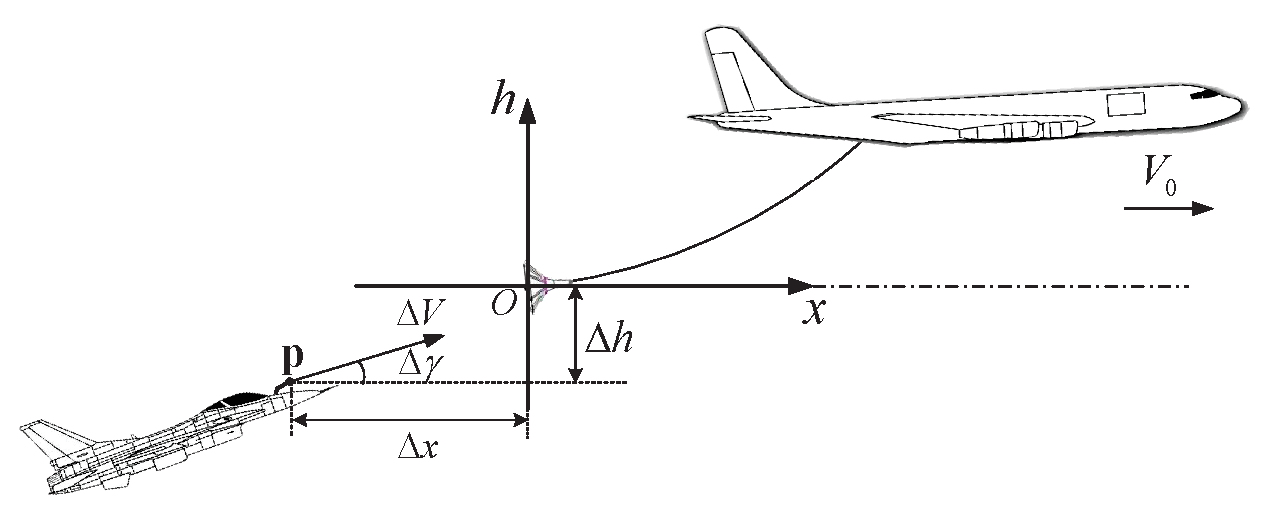
\includegraphics[
		scale=0.5 ]{Figures/Figs_Ch12/pic1.eps}
	\end{center}
	\caption{Relative coordinate system of the docking phase of an AR process}
	\label{figure11}
\end{figure}




The longitudinal dynamics of the receiver aircraft are modeled by using the
reference frame shown in Fig.\ref{figure00}. The receiver aircraft is
subject to the force of thrust $T$, lift $L$, drag $D$ and gravity $G$. The
state vector is $\mathbf{x}_\text{r}=[V_\text{r}$ $\gamma_\text{r}\ x_\text{r}\ h_\text{r}]^{T}$,
whose elements represent the speed, flight path angle, longitudinal distance
and altitude of the mass center of the receiver aircraft, respectively. The
control input is $\mathbf{u}=[T_\text{r}\ \alpha_\text{r}]^{T}$ whose elements denote
the thrust and the angle of attack of the receiver aircraft, respectively.
Therefore, the longitudinal dynamics of the mass center of the receiver
aircraft are written as follows \cite{17} \cite{22}:%
\begin{equation}
\left[
\begin{array}{c}
\dot{V}_\text{r}  \\
\dot{\gamma}_\text{r} \\
\dot{x}_\text{r} \\
\dot{h}_\text{r}%
\end{array}
\right] =\left[
\begin{array}{c}
\frac{1}{m}\left( T_\text{r}\cos \alpha_\text{r}-D\left( \alpha_\text{r},V_\text{r}\right)
-mg\sin \gamma_\text{r}\right) \\
\frac{1}{mV_\text{r}}\left( T_\text{r}\sin \alpha_\text{r}+L\left( \alpha_\text{r},V_\text{r}\right)
-mg\cos \gamma_\text{r}\right) \\
V_\text{r}\cos \gamma_\text{r} \\
V_\text{r}\sin \gamma_\text{r}%
\end{array}
\right] .  \label{0}
\end{equation}

\begin{figure}[htb]
	\begin{center}
		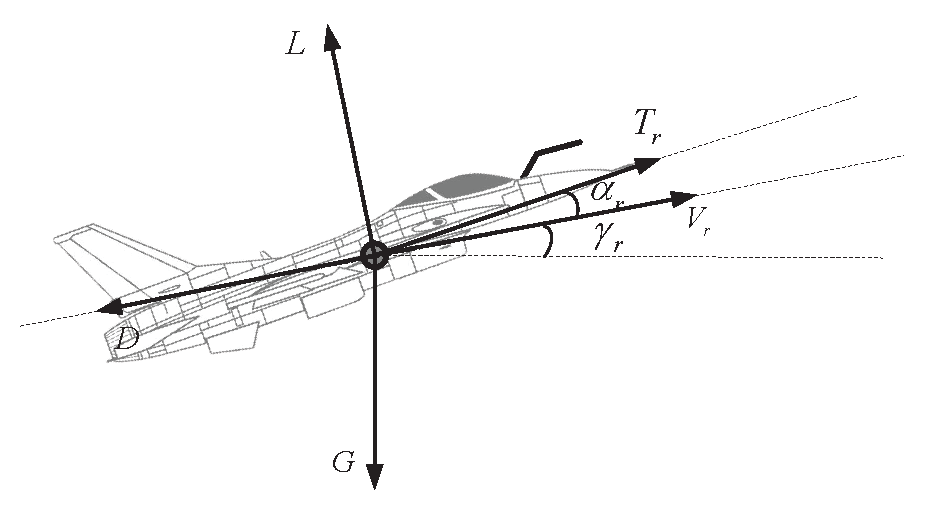
\includegraphics[
		scale=0.55 ]{Figures/Figs_Ch12/pic0.eps}
	\end{center}
	\caption{Longitudinal dynamics of the receiver aircraft}
	\label{figure00}
\end{figure}
The state vector of the tanker aircraft is $\mathbf{x}_\text{t}=[V_\text{t}\ \gamma
_\text{t}\ x_\text{t}\ h_\text{t}]^{T}$, the elements of which represent the speed, the
flight path angle, longitudinal distance and the altitude of the tanker
aircraft, respectively. The state parameters $V_\text{t},h_\text{t}$ are assumed to be
constant at the docking phase, namely
\begin{equation*}
\dot{V}_\text{t}=0,\dot{x}_\text{t}=V_\text{t},\dot{h}_\text{t}=0.
\end{equation*}
This implies $\gamma_\text{t}=0.$ To dock successfully, the receiver aircraft's
speed should keep the same as the tanker aircraft. As a result, the trim
state of the dynamic system Eq.(\ref{0}) is $(V ^{*}\ \gamma ^{*}\ T ^{*}\
\alpha ^{*}),$ where $V ^{*}=V_\text{t},\gamma ^{*}=0.$ Based on the trim state and
input, define%
\begin{align*}
\Delta V_\text{r} & =V_\text{r}-V ^{*},\Delta \gamma_\text{r}=\gamma_\text{r}-\gamma ^{*}, \\
\Delta T_\text{r} & =T_\text{r}-T ^{*},\Delta \alpha_\text{r}=\alpha_\text{r}-\alpha ^{*}.
\end{align*}
Then, Eq.(\ref{0}) is rearranged to%
\begin{equation}
\begin{array}{c}
\underbrace{\left[
	\begin{array}{c}
	\Delta \dot{V}_\text{r}  \\
	\Delta \dot{\gamma}_\text{r} \\
	\Delta \dot{x}_\text{r} \\
	\Delta \dot{h}_\text{r}%
	\end{array}
	\right] } \\
\Delta \mathbf{\dot{x}}_\text{r}%
\end{array}
=%
\begin{array}{c}
\underbrace{\left[
	\begin{array}{c}
	\frac{1}{m}\left(
	\begin{array}{c}
	\left( T ^{*}+\Delta T_\text{r}\right) \cos \left( \alpha ^{*}+\Delta \alpha
	_\text{r}\right) \\
	-D\left( \alpha ^{*}+\Delta \alpha_\text{r},V ^{*}+\Delta V_\text{r}\right) -mg\sin
	\left( \gamma ^{*}+\Delta \gamma_\text{r}\right)%
	\end{array}
	\right) \\
	\frac{1}{m\left( V ^{*}+\Delta V_\text{r}\right) }\left(
	\begin{array}{c}
	\left( T ^{*}+\Delta T_\text{r}\right) \sin \left( \alpha ^{*}+\Delta \alpha
	_\text{r}\right) \\
	+L\left( \alpha ^{*}+\Delta \alpha_\text{r},V ^{*}+\Delta V_\text{r}\right) -mg\cos
	\left( \gamma ^{*}+\Delta \gamma_\text{r}\right)%
	\end{array}
	\right) \\
	\left( V ^{*}+\Delta V_\text{r}\right) \cos \left( \gamma ^{*}+\Delta \gamma
	_\text{r}\right) -V ^{*} \\
	\left( V ^{*}+\Delta V_\text{r}\right) \sin \left( \gamma ^{*}+\Delta \gamma
	_\text{r}\right)%
	\end{array}
	\right] } \\
\mathbf{f}_{h ^{*},V ^{*}}(\Delta \mathbf{x}_\text{r})%
\end{array}
\text{,}  \label{1}
\end{equation}
where the state vector $\Delta \mathbf{x}_\text{r}=[\Delta V_\text{r}$ $\Delta \gamma
_\text{r}\ \Delta x_\text{r}\ \Delta h_\text{r}]^{T}$ represents the speed, flight path
angle, longitudinal distance and altitude of the mass center of the receiver
aircraft with respect to the center of the drogue, respectively. Here, the
lift and drag are expressed as \cite{23}%
\begin{equation}
\begin{array}{c}
L=\frac{1}{2}\rho(V ^{*}+\Delta V_\text{r})^{2}C_{L}S \\
D=\frac{1}{2}\rho(V ^{*}+\Delta V_\text{r})^{2}C_{D}S%
\end{array}
\text{,}  \label{2}
\end{equation}
where $\rho$ is the air density which is determined by the altitude of the
tanker aircraft $h_{0}$ at the docking phase and $S$ represents the wing
area of the receiver aircraft. The lift coefficient $C_{L}$ is a linear
function of $\alpha_\text{r}$ given by%
\begin{equation}
C_{L}=C_{L_{0}}+C_{L_{\alpha}}(\alpha ^{*}+\Delta \alpha_\text{r})\text{,}
\label{3}
\end{equation}
where $C_{L_{0}}$ is the lift coefficient at zero angle of attack and $%
C_{L_{\alpha}}$ is the lift coefficient slope. The drag coefficient $C_{D}$
is computed by the following equation%
\begin{equation}
C_{D}=C_{D_{0}}+KC_{L}^{2}\text{,}  \label{4}
\end{equation}
where $C_{D_{0}}$ is the zero lift drag coefficient which accounts for the
drag of the body, the slats, the flags and the landing gear. The constant $K$
is the lift-induced drag coefficient. According to Eqs.(\ref{2})(\ref{3})(%
\ref{4}), the lift and drag depend on the parameters $V_{0}$ and $h_{0}$. It
implies that the speed and altitude of the tanker aircraft affect the lift
and drag of the receiver aircraft, and further determine the dynamic model
represented by Eq.(\ref{1}).
\begin{figure}[htb]
	\begin{center}
		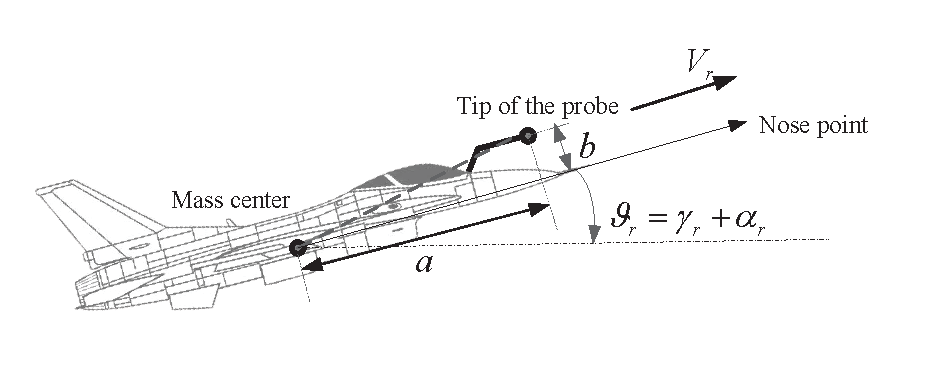
\includegraphics[
		scale=0.6 ]{Figures/Figs_Ch12/pic2.eps}
	\end{center}
	\caption{Relative position of the tip of the probe with respect to the mass
		center of the receiver aircraft}
	\label{figure22}
\end{figure}

\subsection{Assumptions and Objective}

The relative position between the tip of the probe and the mass center of
the receiver aircraft is presented in Fig.\ref{figure22}. As shown, $%
\vartheta _\text{r}$ is the angle of pitch, $a$ and $b$ represent the relative
longitudinal distance and the relative altitude of the tip of the probe with
respect to the mass center of the receiver aircraft. The relative position
between the tip of the probe and the center of the drogue is%
\begin{equation}
\begin{array}{c}
\Delta x=\Delta x_\text{r}+(a\cos \vartheta_\text{r}-b\sin \vartheta_\text{r}) \\
\Delta h=\Delta h_\text{r}+(a\sin \vartheta_\text{r}+b\cos \vartheta_\text{r})%
\end{array}
.  \label{6}
\end{equation}

The following assumptions are further made.

\textbf{Assumption 1.} At the docking phase, the control inputs of the
receiver aircraft are limited by%
\begin{equation}
\begin{array}{c}
\Delta T_{\min}\leq \Delta T_\text{r}\leq \Delta T_{\max} \\
\Delta \alpha_{\min}\leq \Delta \alpha_\text{r}\leq \Delta \alpha_{\max}%
\end{array}
.  \label{7}
\end{equation}

\textbf{Assumption 2. }The speed and the flight path angle of the tip of the
probe are equal to those of the receiver aircraft, given by%
\begin{equation}
\begin{array}{c}
\Delta V=\Delta V_\text{r} \\
\Delta \gamma=\Delta \gamma_\text{r}%
\end{array}
.  \label{16}
\end{equation}

\textbf{Remark 1. }The pilot of the manned aircraft or the UAV autopilot
cannot change the control inputs aggressively during the docking phase.
Thus, \textit{Assumption 1} is reasonable. At the docking phase, the pitch
rate is small. Consequently, its effect on the speed and the flight path
angle of the probe is ignored. Thus, \textit{Assumption 2} is also
reasonable.

According to Eqs.(\ref{6})(\ref{16}), the relative motion between the center
of the drogue and the tip of the probe is expressed as%
\begin{equation}
\Delta \mathbf{x}=\mathbf{g}(\Delta \mathbf{x}_\text{r}).  \label{outputeq}
\end{equation}
Based on the \textit{Assumptions 1-2}, the objective of this paper is to
study the optimal trim state, including the optimal altitude and speed of
the tanker aircraft at the docking phase by using the reachability analysis
method. The optimal altitude and speed will be used to determine the trim
state of the dynamic model described by Eq.(\ref{1}). The docking speed and
altitude of the tanker aircraft corresponding to the maximum volume of the
reachable set is regarded as the optimal speed and altitude at the docking
phase.

\section{Computing Procedure of the Optimal Trim State}

For the docking phase of the AR process, the target set represents the state
set of docking successfully and the reachable set is the state set of the
receiver aircraft from which the docking phase can be completed within a
finite time horizon $t\in \lbrack-\tau,0]$. The target set $\mathcal{D}$ and
the reachable set $pr{{e}_{\tau}}(\mathcal{D})$ can be regarded as the zero
level set of the cost function $J(\mathbf{x},t)$ at $t=0\ $and $t=-\tau$,
respectively. The reachable set $pr{{e}_{\tau}}(\mathcal{D})$ is computed by
solving the following Hamilton-Jacobi Partial Differential Equation (HJ PDE)
\cite{14}%
\begin{equation}
\begin{array}{c}
{{D}_{t}}J(\mathbf{x},t)=-H(\mathbf{x},{{D}_{\mathbf{x}}}J(\mathbf{x},t))\
\\
\ \ \ \ \ \ \ \ \ \ \ \ \ \mathbf{x}\in \mathcal{X},t<0 \\
J(\mathbf{x},0)={{J}_{0}}(\mathbf{x}),\text{ }t=0%
\end{array}
\label{31}
\end{equation}
backward from $t=0$ until $H(\mathbf{x},{{D}_{\mathbf{x}}}J(\mathbf{x}%
,t))\approx0$ or $t=-\tau$ and ${{D}_{t}}J(\mathbf{x},t)$ represents the
derivative of the cost function $J(\mathbf{x},t).$ All the states of the
target set $\mathcal{D}$ and the reachable set $pr{{e}_{\tau}}(\mathcal{D})$
are restricted by the state constraint set $\mathcal{X}$.

For the problem considered in this paper, the target set with respect to $%
\Delta \mathbf{x}$ showing in Fig.\ref{figure11} can be expressed as
\begin{equation}
\mathcal{D}_\text{x}=\{ \Delta \mathbf{x\in}%
%TCIMACRO{\U{211d} }%
%BeginExpansion
\mathbb{R}
%EndExpansion
^{4}\mathbf{|}{J}(\Delta \mathbf{x,}0)\leq0\}.  \label{targetset_y}
\end{equation}
Based on Eq.(\ref{outputeq}), the target set with respect to $\Delta \mathbf{%
	x}_\text{r}$ can be written as
\begin{equation}
\mathcal{D}_{x_\text{r}}=\{ \Delta \mathbf{x}_\text{r}\mathbf{\in}%
%TCIMACRO{\U{211d} }%
%BeginExpansion
\mathbb{R}
%EndExpansion
^{4}\mathbf{|}{J}(\mathbf{g}(\Delta \mathbf{x}_\text{r}),0)\leq0\}.
\label{targetset_x}
\end{equation}
Through Eq.(\ref{targetset_x}), the target set has been transformed into the
range of states $\Delta \mathbf{x}_\text{r}$. Thus, the dynamic model $\Delta
\mathbf{\dot{x}}_\text{r}=\mathbf{f}_{h_{0},V_{0}}(\Delta \mathbf{x}_\text{r})$
described in Eq.(\ref{1}) is adopted to compute the volume of the reachable
set.

Given altitude and speed $(h_{0},V_{0})$ of the tanker aircraft at the
docking phase, the cost function $J(\mathbf{x},t)$ is rewritten as%
\begin{equation}
J(\Delta \mathbf{x}_\text{r},t,h_{0},V_{0})=J(\Delta \mathbf{x}%
_\text{r},t)|_{h_{0},V_{0}}.  \label{18}
\end{equation}
The reachable set is denoted as%
\begin{equation}
\Phi(h_{0},V_{0})=\{ \Delta \mathbf{x}_\text{r}\in \mathcal{X}_\text{r}|J(\Delta
\mathbf{x}_\text{r},t,h_{0},V_{0})\leq0,-\tau \leq t\leq0\},  \label{19}
\end{equation}
where $\mathcal{X}_\text{r}$ represents the state constraint set of the docking
phase.

The volume of the reachable set with respect to $(h_{0},V_{0})$ is defined by%
\begin{equation}
\varphi(h_{0},V_{0})=\left \vert \Phi(h_{0},V_{0})\right \vert ,  \label{20}
\end{equation}
where $\left \vert \cdot \right \vert $ represents the volume of the
reachable set. The relationship between the trim state $(h_{0},V_{0})$ of
the tanker aircraft and the volume of the reachable set is shown in Fig.\ref%
{figure55}. The docking speed $V_{0\text{ }}$and altitude $h_{0\text{ }}$%
affect the volume of the reachable set through determining the trim state of
Eq.(\ref{1}).
\begin{figure}[ptb]
	\begin{center}
		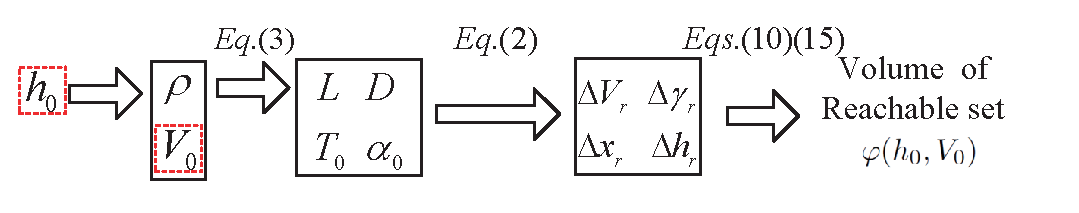
\includegraphics[
		scale=0.4 ]{Figures/Figs_Ch12/pic9.eps}
	\end{center}
	\caption{Relationship between the docking speed $V_{0\text{ }}$docking
		altitude $h_{0}$ and the volume of reachable set $\protect\varphi%
		(h_{0},V_{0})$ }
	\label{figure55}
\end{figure}

The objective of this paper is to obtain the optimal trim state of the
tanker aircraft at the docking phase. The optimal problem is transformed to
find the optimal altitude and speed of the tanker aircraft to maximize the
corresponding volume of the reachable set. The optimization problem is
formulated as%
\begin{equation}
\underset{h_{0}\in \lbrack{{h}_{\min}},{{h}_{\max}}],V_{0}\in \lbrack{{V}%
		_{\min }},{{V}_{\max}}]}{\max}\varphi(h_{0},V_{0}),  \label{12}
\end{equation}
where $\varphi(h_{0},V_{0})$ is defined in Eq.(\ref{20}). In the computing
procedure, the reachable set is calculated on each grid of the continuous
state space $\mathcal{X}_\text{r}$. The value $J(\Delta \mathbf{x}%
_\text{r},t,h_{0},V_{0})$ of each grid of the reachable set is negative,\ thus
the volume of the reachable set is measured by the number of negative grids
in the state space$\mathcal{\ X}_\text{r}$. Thus, the optimal target is rewritten
as%
\begin{equation}
\underset{h_{0}\in \lbrack{{h}_{\min}},{{h}_{\max}}],V_{0}\in \lbrack{{V}%
		_{\min }},{{V}_{\max}}]}{\max}\bar{\varphi}(h_{0},V_{0}),  \label{25}
\end{equation}
where $\bar{\varphi}(h_{0},V_{0})$ is a function representing the number of
negative grids. The optimal solution to Eq.(\ref{25}) can be seen as the
approximate solution of Eq.(\ref{12}), namely%
\begin{align}
(h_\text{op},V_\text{op}) & =\arg \underset{h_{0}\in \lbrack{{h}_{\min}},{{h}_{\max}}%
	],V_{0}\in \lbrack{{V}_{\min}},{{V}_{\max}}]}{\max}\varphi(h_{0},V_{0})
\label{32} \\
& \approx \arg \underset{h_{0}\in \lbrack{{h}_{\min}},{{h}_{\max}}],V_{0}\in
	\lbrack{{V}_{\min}},{{V}_{\max}}]}{\max}\bar{\varphi}(h_{0},V_{0}).  \notag
\end{align}

The simulation time step is set to $\Delta t=0.1s$ and the backward
computation time is $t=-i\times \Delta t$, $i=1,2...,10$. The computing
procedure of the optimal trim state of the tanker aircraft is presented as
follows:

\textit{Step1}. Initialize the state space, target set and the corresponding
grid points.

\textit{Step2}. For the specified docking altitude $h_{0}$ and docking speed
$V_{0}$, calculate $T_{0}$ and $\alpha_{0}.$

\textit{Step3}. Repeat

Solve the HJ PDE (\ref{31}) at each backward
computation time $t=-i\times \Delta t$\ to get the reachable set

until $t=-1s$ or $H(\mathbf{x},D_{\mathbf{x}}J(\mathbf{%
	x},t))\approx0.$

\textit{Step4}. Calculate the volume of the reachable set for the selected
docking altitude $h_{0}$ and docking speed $V_{0}$ according to $\bar{\varphi}%
(h_{0},V_{0}). $

\textit{Step5}. Obtain the optimal docking altitude $h_\text{op}$ and speed $%
V_\text{op}$ which correspond to the maximum volume of the reachable set.

\section{Simulation analysis on the Optimal Docking Altitude and Speed of
	F-16 aircraft}

\subsection{Simulation Description}

A simplified nonlinear F-16 aircraft model is used to compute the optimal
trim state based on the computing procedure proposed in Section III. In this
section, the system parameters of Eq.(\ref{1}), the control constraint set,
the state constraint set, the target set at the docking phase are provided.

\textbf{(i) System Parameters.} The physical parameters of the F-16 aircraft
model are shown in Table \ref{Physical_parameters}. The related parameters
used in Eq.(\ref{1}) are given in Table \ref{related parameters}. The lift
coefficient $C_{L}$ and drag coefficient $C_{D}$ are obtained through the
linear interpolation in the lift curve and drag curve of the F-16 aircraft
\cite{17}.

\textbf{(ii) Control Constraint Set.} As presented in Section II, $%
T_\text{r}=T ^{*}+\Delta T_\text{r}$ and $\alpha_\text{r}=\alpha ^{*}+\Delta \alpha_\text{r}$. As
shown in Fig.\ref{figure55}, $T_{0}$ and $\alpha_{0}$ are determined by the
trim state $(h_{0},V_{0})$ of the tanker aircraft. The limits of the control
inputs of the Eq.(\ref{1}) are provided in Table \ref{control limits}.

\textbf{(iii) State Constraint Set. }The Cartesian grid is used to
approximate the state space $\mathcal{X}_\text{r}$. The ranges of the states of
the system and the grid division are shown in Table \ref{Grid division}. If
the states are out of the ranges, then the docking is considered to fail.

\textbf{(iv) Target Set.} A neighborhood around the desired final states at
the docking phase is chosen as the target set. For the considered system,
the target set with respect to $\Delta \mathbf{x}$ is%
\begin{equation}
\mathcal{D}_\text{x}=\left\{ \left.\Delta\mathbf{x\in}%TCIMACRO{\U{211d}}%
%BeginExpansion
\mathbb{R}%EndExpansion
^{4}\right\vert {J}(\Delta\mathbf{x,}0)=\max\left(\begin{array}{l}
\max\mathbf{(}\Delta\tilde{V}-\Delta V_\text{up},\Delta V_\text{low}-\Delta\tilde{V}),\\
\max(\Delta\tilde{\gamma}-\Delta\gamma_\text{up},\Delta\gamma_\text{low}-\Delta\tilde{\gamma}),\\
\max(\Delta\tilde{x}-\Delta x_\text{up},\Delta x_\text{low}-\Delta\tilde{x}),\\
\max(\Delta\tilde{h}-\Delta h_\text{up},\Delta h_\text{low}-\Delta\tilde{h})
\end{array}\right)\leq0\right\} ,\label{TargetDP}
\end{equation}
where $\Delta \mathbf{\tilde{x}}=[\Delta \tilde{V}\ \Delta \tilde{\gamma}\
\Delta \tilde{x}\ \Delta \tilde{h}]^{T}$ represents the state vector of each
grid point and $\Delta V_\text{up}=2{m}/{s,}$ $\Delta V_\text{low}=-0.2{m}/{s,}$ $%
\Delta \gamma_\text{up}={{0.5}^{\circ},}$ $\Delta \gamma_\text{low}=-{{0.5}^{\circ},}$
$\Delta x_\text{up}=0m,$ $\Delta x_\text{low}=-0.3m,$ $\Delta h_\text{up}=1m,$ $\Delta
h_\text{low}=-1m\ $which represent the upper and lower boundary of the target
set. Based on Eq.(\ref{TargetDP}), the target set can be rewritten as
\begin{equation}
\mathcal{D}_\text{x}=\left \{ \left. \Delta \mathbf{x\in}%
%TCIMACRO{\U{211d} }%
%BeginExpansion
\mathbb{R}
%EndExpansion
^{4}\right \vert
\begin{array}{c}
-0.2{m}/{s}\leq \Delta V\leq2{m}/{s},-{{0.5}^{\circ}}\leq \Delta \gamma \leq
{{0.5}^{\circ}}, \\
-0.3m\leq \Delta x\leq0m,-1m\leq \Delta h\leq1m%
\end{array}
\right \} .  \label{14}
\end{equation}
\begin{table}[ptb]
	\caption{Physical parameters of F-16 aircraft model}
	\label{Physical_parameters}%
	%\begin{ruledtabular}
	\centering%
	\begin{tabular}{c|c|c|c}
		\hline\hline
		Parameters & $m$ & $g$ & $S$ \\ \hline
		Value & 20500 lbs & 9.8 $m/s^{2}$ & 300 ft$^{2}$ \\ \hline\hline
	\end{tabular}%
\end{table}
\begin{table}[ptb]
	\caption{Related parameters of dynamic model}
	\label{related parameters}%
	%\begin{ruledtabular}
	\centering%
	\begin{tabular}{c|c|c|c|c|c|c}
		\hline\hline
		Parameters & $C_{L_{0}}$ & $C_{L_{\alpha}}$ & $C_{D_{0}}$ & $K$ & $a$ & $b$
		\\ \hline
		Value & 0.1 & 0.06 & -0.021 & 0.35 & 3$m$ & 0.5$m$ \\ \hline\hline
	\end{tabular}
	%\end{ruledtabular}
\end{table}
\begin{table}[ptb]
	\caption{Limits of the variations of the control inputs of the dynamic model}
	\label{control limits}%
	%\begin{ruledtabular}
	\centering%
	\begin{tabular}{l|c|c}
		\hline\hline
		Variations of the control inputs & Min & Max \\ \hline
		$\ \ \ \ \ \ \ \ \ \ \ \ \ \ \ \ \ \ \Delta T_\text{r}$ & -2000N & 2000N \\ \hline
		$\ \ \ \ \ \ \ \ \ \ \ \ \ \ \ \ \ \ \Delta \alpha_\text{r}$ & -2${{}^{\circ}}$ &
		2${{}^{\circ}}$ \\ \hline\hline
	\end{tabular}
	%\end{ruledtabular}
\end{table}
\begin{table}[ptb]
	\caption{Grid division of the state space}
	\label{Grid division}%
	%\begin{ruledtabular}
	\centering%
	\begin{tabular}{l|cccc}
		\hline\hline
		Parameters & $\Delta V_\text{r}(m/s)$ & $\Delta \gamma_\text{r}(\deg)$ & $\Delta
		x_\text{r}(m)$ & $\Delta h_\text{r}(m)$ \\ \hline
		Range & [-2,7] & [-10,5] & [-4,0.5] & [-1,1] \\ \hline
		Grid numbers & 40 & 30 & 20 & 20 \\ \hline
		Step size & 0.23 & 0.5 & 0.23 & 0.1 \\ \hline\hline
	\end{tabular}
	%\end{ruledtabular}
\end{table}
At the docking phase $\gamma_\text{t}$ and $\gamma_\text{r}$ approach zero degree,
namely $\gamma_\text{t}=\gamma_\text{r}\approx0^{\circ}$. Thus, in Fig.\ref{figure22},
$\vartheta_\text{r}\approx \alpha_\text{r}$. The parameter $\alpha_\text{r}$ is small$\ $at
the docking phase leading to $\vartheta_\text{r}\approx0^{\circ}.$ Through the
transformation of Eq.(\ref{targetset_x}), the target set specified in the
relative coordinate system is expressed by
\begin{equation}
\mathcal{D}_{x_\text{r}}=\left\{ \left.\Delta\mathbf{x}_\text{r}\mathbf{\in}%TCIMACRO{\U{211d}}%
%BeginExpansion
\mathbb{R}%EndExpansion
^{4}\right\vert \begin{array}{l}
-0.2{m}/{s}\leq\Delta V_\text{r}\leq2{m}/{s},\\
-{{0.5}^{\circ}}\leq\Delta\gamma_\text{r}\leq{{0.5}^{\circ}},\\
(-0.3-a)m\leq\Delta x_\text{r}\leq(-a)m,\\
(-1-b)m\leq\Delta h_\text{r}\leq(1-b)m
\end{array}\right\} ,\label{33}
\end{equation}
where the target set $\mathcal{D}_{x_\text{r}}$ is a small hypercube.

\textbf{Remark 2. }The target set is a four-dimensional (4D) hypercube. So,
the function ${J}(\Delta \mathbf{x,}0)$ in Eq.(\ref{TargetDP}) is not
differentiable. However, the HJ PDE can be still solved by a numerical
method. According to Eq.(\ref{TargetDP}), the distance between each grid
point and the boundary of the target set can be obtained by the function
"shapeRectangleByCorners" in the ToolboxLS \cite{20}. For the discrete grid
points, the derivative of $J(\Delta \mathbf{x}_\text{r},t)|_{h_{0},V_{0}}$ can be
computed.

\textbf{Remark 3. }The primary weakness of the reachability analysis method
is that memory and computational time requirements rise exponentially with
dimension. In practice, systems of dimensions 1$\sim$3 can be
examined interactively \cite{14}. The dimension of the longitudinal dynamics
of the mass center of the receiver aircraft is four. It is slow but feasible
on a computer with sufficient memory. Since the exact computation of
reachable set is typically done off-line, the over-approximating reachable
set can allow for real-time computation\ \cite{15}.

\subsection{Optimal docking speed and docking altitude}

\begin{figure}[ptb]
	\begin{center}
		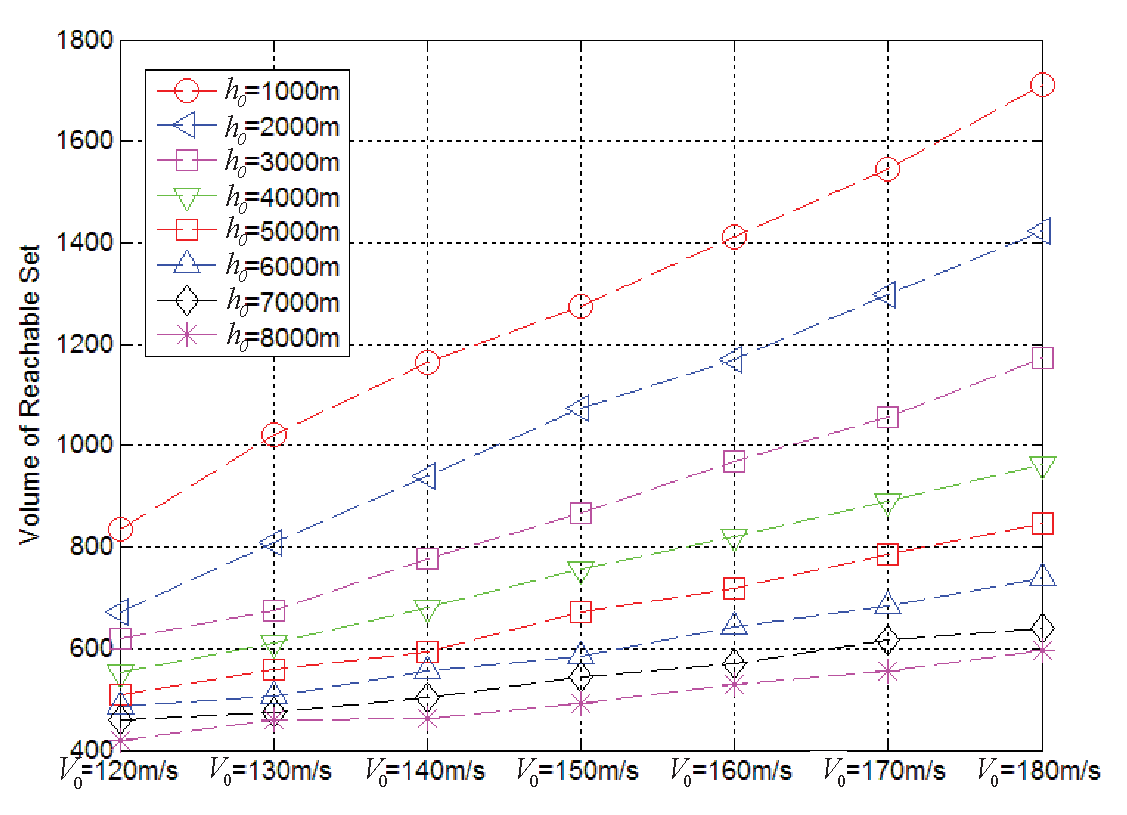
\includegraphics[
		scale=0.6 ]{Figures/Figs_Ch12/pic5.eps}
	\end{center}
	\caption{Volume of reachable set at different altitudes and different
		docking speeds}
	\label{figure66}
\end{figure}

In this section, the volumes of the reachable set at different docking
altitudes and speeds are depicted in Fig.\ref{figure66}. The computation of
reachable set is typically done off-line in Matlab, and run on a desktop
with 2.4GHz CPU and 2GB RAM. The computation time is 986.878 seconds at each
discrete altitude and speed. Furthermore, the computation time of the
volumes of the reachable set is 0.000046s. The Matlab source code of the
paper is presented in our research group website
http://rfly.buaa.edu.cn/resources/. The altitude and speed of the F-16
aircraft at the docking phase is confined to $1000$m$\thicksim8000$m with
the interval $1000$m and $120$m/s$\thicksim 180$m/s with the interval $10$%
m/s, respectively. The volume of the reachable set at discrete altitude and
speed is%
\begin{equation}
\begin{array}{l}
RS_{ij}=\bar{\varphi}(h(i),V(j)) \\
h(i)=1000+1000\ast i,\text{ }i=0,1,2,...,7 \\
V(j)=120+10\ast j,\text{ }j=0,1,2,...,6%
\end{array}
.  \label{26}
\end{equation}

\begin{figure}[ptb]
	\begin{center}
		\includegraphics[
		scale=0.4 ]{Figures/Figs_Ch12/pic7.eps}
	\end{center}
	\caption{Target set (green) and reachable set (red) for three-dimensional
		(3D) slices of the four-dimensional (4D) reachable set with the optimal
		altitude $h_\text{op}=1000m$ and the optimal docking speed $V_\text{op}=180m/s$. }
	\label{figure77}
\end{figure}
From the obtained results in Fig.\ref{figure66}, three observations can be
concluded. (i) As the altitude changes from $1000$m to $8000$m, the volume
of the reachable set $\bar{\varphi}(h_{0},V_{0})$ is monotonously decreased.
(ii) The volume of the reachable set $\bar{\varphi}(h_{0},V_{0})$ at a high
altitude is always small regardless of the docking speed. (iii) As the speed
changes from $120$m/s to $180$m/s, the volume of the reachable set $\bar{%
	\varphi}(h_{0},V_{0})$ is monotonously increased. This implies that the
faster the tanker aircraft is, the bigger state space the receiver aircraft
can be operated in. Then, the optimal docking altitude $h_\text{op}$ and optimal
speed $V_\text{op}$ are obtained by%
\begin{equation}
(h_\text{op},V_\text{op})=\arg \underset{h_{0}\in \lbrack{{h}_{\min}},{{h}_{\max}}%
	]V_{0}\in \lbrack{{V}_{\min}},{{V}_{\max}}]}{\max}\bar{\varphi}(h_{0},V_{0})%
\text{.}  \label{30}
\end{equation}
They are $h_\text{op}=1000$m and $V_\text{op}=180$m/s. The corresponding maximum
volume of the reachable set is $\bar{\varphi}(h_\text{op},V_\text{op})=1710$.



The reasons for these observations are summarized as follows. (i) As the
altitude is increased, the air density is decreased. Therefore, the receiver
aircraft should increase the speed to balance the gravity and the drag
force. Meanwhile, the maneuverability of the aircraft becomes worse at a
high altitude, resulting in a small volume of the reachable set. (ii) The
air density is increased as the altitude is decreased, and the
maneuverability of the aircraft becomes better. Thus, the corresponding
volume of the reachable set is bigger. This implies that it is suitable for
docking at a low altitude. However, by considering the air turbulence and
the operational risk of the pilots, it is better to dock at a medium
altitude and a medium speed for safety considerations.


\begin{figure}[ptb]
	\begin{center}
		\includegraphics[
		scale=0.6]{Figures/Figs_Ch12/pic10.eps}
	\end{center}
	\caption{For different matrix $\mathbf{Q}$ and $\mathbf{R}$, the numbers of
		docking success grid at different altitudes and speeds}
	\label{figure88}
\end{figure}

The further explanation is provided as follows. The maneuverability is
roughly related to the feasible control input of an aircraft. The larger the
maneuverability, the more margin the feasible control can offer, implying a
larger reachability roughly\ \cite{25}. Compared with the maneuverability,
the proposed reachability is more exact as it has taken both control input
and the system dynamics into consideration. Often, the maneuverability of an
aircraft is measured by the normal load factor $n_{y}$ which can be
expressed as $n_{y}=L/G$. The gravity $G$ is constant. If the lift $L$ is
larger, its corresponding normal load $n_{y}$ is larger, i.e., the
maneuverability is better. According to the Fig.\ref{figure66}, two cases
are considered. In the first case, the speed $V$ is set to be constant and
the altitude $h_{1}$ is set to be higher than the altitude $h_{2}$ which are
both between $1000$m and $8000$m$.$ The air densities at the altitudes $%
h_{1} $ and $h_{2}$ are supposed to be $\rho_{1}$ and $\rho_{2}$,
respectively. The formula of the Mach number is $M=V/V_{a},$ where $V_{a}$
represents the speed of sound. The Mach number at the altitude $h_{1}$ and $%
h_{2}$ are set to be $M_{1}$ and $M_{2}$, respectively. According to the
formula of the lift $L\ $which has been provided in Eq.(\ref{2}), the lift
at the altitude $h_{1}$ and $h_{2}$ can be expressed as $L_{1}=\frac{1}{2}%
\rho_{1}V^{2}C_{L_{1}}S$ and $L_{2}=\frac{1}{2}\rho_{2}V^{2}C_{L_{2}}S$. As
the altitude is increased, the air density $\rho$ is decreased, namely $%
\rho_{1}<\rho_{2}$. Meanwhile, the speed of sound $V_{a}$ is also decreased,
implying the Mach number $M_{1}>M_{2}$ and the corresponding lift
coefficient $C_{L_{1}}<C_{L_{2}}$. Thus, the lift $L_{2}$ is larger than the
lift $L_{1}$ and then the maneuverability at the altitude $h_{2}$ is better.
This means that if the aircraft speed $V$ is constant, then the volumes of
the reachable set at altitude $h_{2}$ is larger because the maneuverability
at the altitude $h_{2}$ is better.\ In the second case, the altitude $h$ is
set to be constant and the speed $V_{1}$ is set to be larger than the speed $%
V_{2}$ which are both between $120$m/s$\ $and $180$m/s. According to the
definition of the lift $L$, the lifts at the speed $V_{1}$ and the speed $%
V_{2}$ can be expressed as $L_{1}=\frac{1}{2}\rho V_{1}^{2}C_{L}S$ and $%
L_{2}=\frac{1}{2}\rho V_{2}^{2}C_{L}S$, respectively. It is obvious that the
lift $L_{1}$ is larger than $L_{2}$. This implies that the maneuverability
at the speed $V_{1}$ is better than that at the speed $V_{2}$. Therefore, if
the aircraft altitude $h$ is set to be constant, then the volume of the\
reachable set at speed $V_{1}$ is larger than that at the speed $V_{2}$.

The Fig.\ref{figure77} shows the 3D slices of the 4D maximum reachable set.
The 4D maximal reachable set is the largest controllable set from which the
receiver aircraft can dock successfully.




\subsection{Verification}

\subsubsection{Verification by using LQR controllers}



In this section, LQR controllers are used to verify the optimal trim state
at the docking phase. It is reasonable to adopt LQR controller to verify the
simulation results owing the fact that LQR approach is often employed to
design the docking control laws for the AR process\ \cite{3} \cite{26} \cite{27}. The number of docking success grids of the reachable set at
different altitudes and speeds within a specified time horizon is used to
measure how difficult the docking is. If the number is larger, it means that
it is easier to dock with the corresponding controller. The main steps of
verification are shown as follows:



\textit{Step1}. Calculate $T_{0}$ and $\alpha_{0}$ at the docking altitude $%
h_{0}$ and docking speed $V_{0}$.

\textit{Step2}.\ Linearize the dynamic model of the system as in Eq.(\ref{1}%
) which is written as
\[
\Delta\mathbf{\dot{x}}_\text{r}=\mathbf{A}_\text{r}\Delta\mathbf{x}_\text{r}+\mathbf{B}_\text{r}\mathbf{u},
\]
where
\[
\begin{array}{c}
\mathbf{A}_{r}=\left[\begin{array}{cccc}
-\frac{\rho V_{0}SC_{d}}{m} & -g\cos\gamma_{0} & 0 & 0\\
\frac{\frac{1}{2}\rho V_{0}^{2}SC_{L}-T_{0}\sin\alpha_{0}+mg\cos\gamma_{0}}{mV_{0}^{2}} & \frac{g\sin\gamma_{0}}{V} & 0 & 0\\
\cos\gamma_{0} & -V_{0}\sin\gamma_{0} & 0 & 0\\
\sin\gamma_{0} & V_{0}\cos\gamma_{0} & 0 & 0
\end{array}\right],\\
\mathbf{B}_\text{r}=\left[\begin{array}{cc}
\frac{-T_{0}\sin\alpha_{0}}{m} & \frac{\cos\alpha_{0}}{m}\\
\frac{-T_{0}\cos\alpha_{0}}{mV_{0}} & \frac{\sin\alpha_{0}}{mV_{0}}\\
0 & 0\\
0 & 0
\end{array}\right].
\end{array}
\]

\textit{Step3}. Each grid point of the reachable set at the selected docking
altitude $h_{0}$ and docking speed $V_{0}$ is taken as the initial state of
the LQR controllers (see the \textit{Appendix }for details). The controllers
are used to drive the state of the receiver aircraft into\ the target set $%
\mathcal{D}$. The control time is set to be 5s, which is longer than the
backward computation time of the reachable set. This is because the LQR\
controllers need enough time to converge.

\textit{Step4}. Record the number of docking success grid of the reachable
set which can be defined as $\tilde{\varphi}(h_{i},V_{j})$ at different
altitudes and speeds.

The numbers of docking success grid for three LQR controllers are depicted
in Fig.\ref{figure88}. As shown, two observations can be concluded. (i) The $%
\tilde{\varphi}(h_{i},V_{j})$ is proportional with $\bar{\varphi}%
(h_{i},V_{j})$. (ii) The maximum number of the docking success grid for
different LQR controllers are $1207$, $1353$ and $1708$ with altitude $%
h_{i}=1000$m and docking speed $V_{j}=180$m/s which corresponds with the
maximum volume of the reachable set. The verification of the results leads
to the following conclusions. (i) The success rate of the LQR controller is
proportional with the volume of reachable set. (ii) It is more suitable to
design controllers at the optimal trim state at the docking phase.

\subsubsection{Verification by using degree of controllability}

In this section, a degree of controllability (DoC) is adopted to verify the
effectiveness of the proposed method from another aspect. The linear
dynamical model of the system is $\Delta \mathbf{\dot{x}}_\text{r}=\mathbf{A}%
_{r}\Delta \mathbf{x}_\text{r}+\mathbf{B}_\text{r}\mathbf{u,}$ where the control input
$\mathbf{u}=[T_\text{r}\ \alpha_\text{r}]^{T}\in \Omega$. The definitions of recovery
region and DoC are obtained according to \cite{28}.

\textbf{Definition 1}. For the linear dynamical model of the system, the
recovery region $\mathcal{R}$ within time $t_{\text{r}}$ is defined as%
\begin{equation}
\mathcal{R}\left( t_{\text{r}}\right) =\left \{ \Delta \mathbf{x}_\text{r}\left(
0\right) |\exists \mathbf{u}\left( t\right) \in \Omega,t\in \left[ 0,t_{%
	\text{r}}\right] ,\text{s.t. }\Delta \mathbf{x}_\text{r}\left( t_{\text{r}%
}\right) =\mathbf{0}\right \}  \label{recovery_region}
\end{equation}

\textbf{Definition 2}. For the linear dynamical model of the system, the DoC
$\rho$ within time $t_{\text{r}}$ is defined as%
\begin{equation}
\rho_{\text{doc}}=\inf \left \Vert \Delta \mathbf{x}_\text{r}\left( 0\right)
\right \Vert \text{ }\forall \Delta \mathbf{x}_\text{r}\left( 0\right) \notin
\mathcal{R}\left( t_{\text{r}}\right)  \label{doc_definition}
\end{equation}
where $\left \Vert \mathbf{\cdot}\right \Vert $ represents the Euclidean
norm.

From \emph{Definition 2,} it is observed that the minimal distance from the
origin to the boundary of the recovery region is considered to be the DoC of
the system. The value of $\rho_{\text{doc}}$ represents how controllable the
system is. The larger the value of $\rho_{\text{doc}}$, the stronger the
system control ability is. The values of $\rho_{\text{doc}}$ at different
altitudes and speeds can be defined as $\rho_{\text{doc}}(h_{i},V_{j})$
which are shown in Fig.\ref{Doc_2d3d}. As shown in Fig.\ref{Doc_2d3d}, the $%
\rho_{\text{doc}}(h_{i},V_{j})$ is proportional with $\bar{\varphi}%
(h_{i},V_{j})$. This shows the feasibility of our simulation results from
another aspect. The use of DoC is not used to to replace with the
reachability analysis but is only taken as a verification for the
reachability analysis, because i) the target set is only zero rather than a
set as in Eq.(\ref{targetset_x}) for reachability analysis here; ii) a
linear model is used rather than nonlinear model used for the reachability
analysis.
\begin{figure}[ptb]
	\begin{center}
		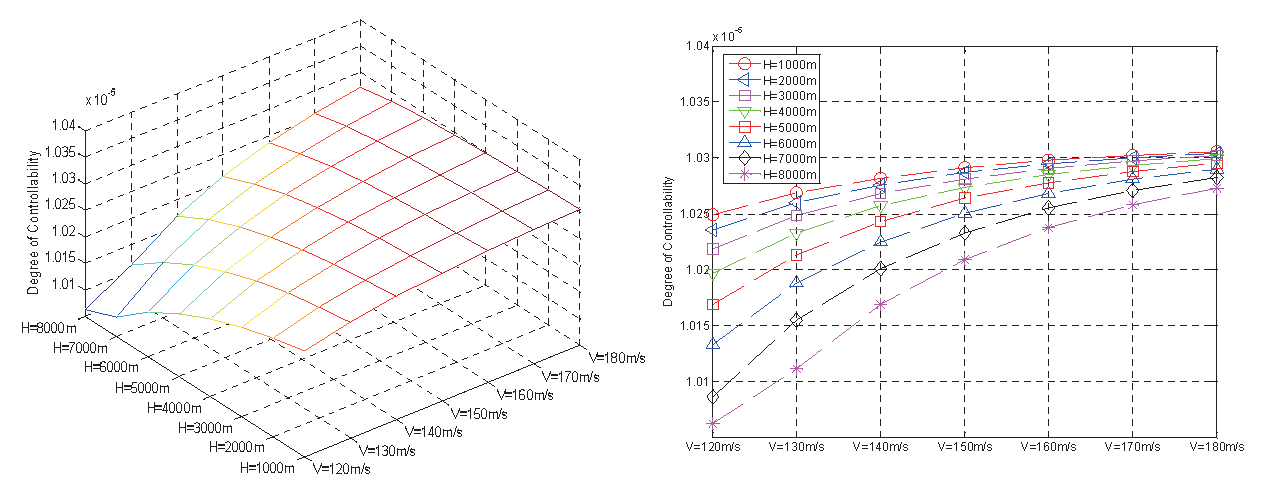
\includegraphics[
		scale=0.6]{Figures/Figs_Ch12/2d3d.eps}
	\end{center}
	\caption{(Left) Three-dimensional surface and (right) two-dimensional curve
		of the value of $\protect\rho_{\text{doc}}$ at different altitudes and
		speeds }
	\label{Doc_2d3d}
\end{figure}

\section{Chapter Summary}

In order to improve the success rate of docking in an AR process, the
reachability analysis method is used to obtain the optimal trim state of the
tanker aircraft at the docking phase. The optimal trim state is defined as
the docking state of the tanker aircraft corresponding to the maximum volume
of the reachable set. First, in order to find the optimal trim state of the
tanker aircraft at the docking phase, 4D relative motion model between the
receiver aircraft and the center of the drogue is proposed. Based on it, a
step-by-step computing procedure to obtain the optimal docking speed and
altitude is proposed. Then, the simulation on a simplified nonlinear F-16
aircraft model is studied comprehensively. From the simulation, the success
rate of the proposed LQR controller is proportional with the volume of the
reachable set so that the proposed method to obtain the optimal trim state
of the tanker aircraft is reasonable. Furthermore, a DoC method is also used
to verify the feasibility of the optimal trim state from another aspect.

For the simulation results, the brute force search method is used to
determine the optimal trim state. From the simulation results obtained, the
problem seems like convex optimization problem. But it is difficult to
verify the convexity of the simulation results, the major reason for which
is the function of the volume of the reachable set is not easy to use an
analytical function to express. But the convexity of the simulation results
is also a problem which is needed to be solved. The verification of its
convexity of the optimization problem is regarded as the further study.

